\documentclass[11pt]{article}
\usepackage[utf8]{inputenc}

\usepackage{amssymb}
\usepackage{amsmath}
\usepackage{amsthm}
\usepackage{graphicx} 
\usepackage{fullpage}
\usepackage[ruled,vlined,linesnumbered]{algorithm2e}

\setlength{\parindent}{0em}  % set the indent of the paragraph
\setlength{\parskip}{0em} % set the space of the paragraph

\theoremstyle{definition}
\newtheorem{definition}{Definition}[section] % add the section number in front of the definition number
% \newtheorem*{definition}{Definition} % remove the index number of the definition

\title{Data	Exploration Project}
\author{Xianlin Feng}
\date{\today}

\begin{document}
\maketitle

\section{Introduction}
Road traffic accident is a threat to all people in their daily life. According to the WHO's statistics in 2018, road traffic accidents are the eighth of the top 10 causes of death, which is the only reason of injuries, and all the remaining reason are diseases. In the worldwide, road injuries took 140 million lives in 2016, in which $74\%$ are were men and boys. (https://www.who.int/news-room/fact-sheets/detail/the-top-10-causes-of-death). Serious situation happened in Victoria too. There were 58 lives lost because of the road accident every day in 2018 just in Victoria. This number increased to 88 since 7 April 2019. In the last five years, the least worse situation happened in 2017, the daily lives lost was 64.  According to the TAC report, the lives lost of drivers takes nearly half ($48.2\%$) of the daily lives lost. The age of death is concentrated in 30-69 years old. The most lives lost in rural roads($58\%$).(http://www.tac.vic.gov.au/road-safety/statistics/lives-lost-year-to-date). The analysis of past traffic accidents can provide a basis for future road construction, accident prevention, and accident rescue. The following three question will be answered in this report:
\begin{enumerate}
	\item What is the main cause of road crashes in Victoria.
	\item What is the trend in the last 10 years?
	\item What suggestion we can provide for the people in different areas.
\end{enumerate}
To answer those three questions, I will try to analysis and explore the dataset to find the main cause of road crashes in Victoria, as well as the trend in the last 10 years. I will try to find one or more datasets, then perform data wrangling, data cleaning and data checking before data exploration. During the data exploration, I will perform different statistic tests and visualisation to explore the data set and obtain insight from the data. At last, I will provide some suggestions base on the result of the data exploration. The main structure of this report is as follow: the data wrangling will be processed in section \ref{dataWrangling}, then the data will be checking in section \ref{dataChecking}. The data exploration will be carried out in section \ref{dataExploration}, followed by the section of conclusion. In the last section, there will be a reflection of this assessment. 
\par


\section{Data Wrangling} 
\label{dataWrangling}
Usually the data we get is messy and incomplete, which cannot be used for data analysis directly. Data wrangling is a process to manipulate data to make the data directly usable for analysis. According to "2016 Data Science Salary Survey",  data scientists spend 53\% of their time for data cleaning and data wrangling. (https://learning.oreilly.com/library/view/2016-data-science/9781492049029/). During the data wrangling, the raw data is transformed into the data that can be analysed to generate insights and valid results. Data wrangling is vital for data science project, which not only improves the efficiency of data analysis, but also reduces the error caused by erroneous data. In this section, I will divide the data wrangling process into the following small tasks base on the characteristics of the data set:
\begin{enumerate}
	\item Introduce the data set
	\item delete expired data
	\item select data
	\item Drop missing or null values in the dataset
	\item Time series data handling	
	\item Filtering Data
	\item Grouping Data
	\item convert free text dates to standard format
	\item deal with outliers or "illegal" values
	\item discrete the data into a set of values
	\item data checking
\end{enumerate}


\subsection{the Dataset}
The data set I found for this project named "CrashStats data", which could be downloaded on Victoria government open data website: https://www.data.vic.gov.au . The dataset was provide by VicRoad for educational purposes, and it includes the crash data of time, location, conditions and so on since 2000. The dataset is consist with 12 tables in the following list:
\begin{enumerate}
	\item \textbf{accident}:	contain the besic information about the accident, such as date, time, location, environment codition and severity.
	\item \textbf{vehicle}:	vehicle information, such as make, body type, year of manufacture, fuel type, vechicle capacity and so on.
	\item \textbf{person}:	person details, such as age, sex, sitting position, passengers or driver, license state etc.	
	\item \textbf{accident$\_$event}: the sequence of events during the accident, such as ran off carriageway, collision, fell from vehicle, and so on.
	\item \textbf{accident$\_$location}:	the location information of the accident.
	\item \textbf{road$\_$surface$\_$cond}:	the codition of the road: wet, dry, or icy.
	\item \textbf{atmospheric$\_$cond}:	weather condition: clear, wind, dust and so on.
	\item \textbf{sub$\_$dca}:	describing the crash detail with code.
	\item \textbf{accident$\_$node}:	more detailed location about the crash.
	\item \textbf{accident$\_$chainage}:	chainage information of the node.
	\item \textbf{node$\_$id$\_$complex$\_$int$\_$id}:	if the node locate in a complex intersection or not.
	\item \textbf{statistic$\_$checks}:	the statistic information of the crashes in this dataset.
\end{enumerate}
Before the data wrangling and data cleaning, we need to understand the characteristics of each data table, for example, in the table of "accident", each accident has exact one record. But, as one accident may involved two or more people, one accident may have two or more records in the table "person". Same situation happens in table "vehicle", "accident$\_$event" and other tables too, this is another reason why this dataset separate to 12 data tables. Due to this reason, when we process data wrangling, data cleaning, or data exploration, extra careful should be paid with the multiple records for one accident. 

\subsection{Filter data}	
\subsection{Delete expired data}
The crash happened more ten years ago is not considered in this report, so they will be delete form the dataset in the first step. Fortunately, every crash in the dataset have a accident number, the accident number consist with the date information and the index number, so the instances before 1/1/2009 and after 31/12/2018 should be delete first in each subset.   This step was performed in Microsoft Excel. Then after deleting the expired data, there are 135226 instance in the data set.

\subsection{Select data}
Another important step after deleting expired data is selecting data. Each data instance contains lots of information related to the accident, however some of them are not related to our project. So that, select the useful data and information is essential for data analysis. This step is performed in Microsoft Excel too, and the data tables still stored in ".csv" format. The list blow indicate the selected attributes for each table:
\begin{enumerate}
	\item \textbf{accident}: accident number, date, time, type, day of week, accident type, light condition, node, involved vehicles, road condition and so on.
	\item \textbf{person}: sex, age, injured level, seating position, role, license information, movement. 
	\item \textbf{vehicle}: register state, make, model, year of manufacture, type, body style, number of person, color, level of damage, collision position. 
	\item \textbf{accident$\_$node}:	node$\_$ID, type, latitude, longitude. postcode.  
	\item \textbf{road$\_$surface$\_$cond}: road surface condition.
	\item \textbf{accident$\_$event}: event sequence, event type, collision position and so on.
	\item \textbf{accident$\_$location}:	 node$\_$ID, type of intersecting road, distance to the nearest intersecting road. 
	\item \textbf{atmospheric$\_$cond}:	atmospheric condition.
\end{enumerate}


\subsection{Time series data handling}
In the original data set, the time information is stored in the format \text{"hh.mm.ss"}, which is not the common time format, so that I change them to the format \text{"hh:mm:ss"} first. This step could easily perform in Microsoft Excel by just replacing every "." by ":". Then, the date and time information are separated into two columns, which is not very friendly to Tableau Public, so we need to combine them together first. In order to complete this task, I need to use a Excel formulation \text{"TEXT(B2,"d\/mm\/yyyy")\&" "\&TEXT(C2,"hh:mm:ss")"}. This formulation could combine the date information in cell "B2" and time information in cell "C2" without lose any information. By applying this formulation to all rows, a new column that contain both date and time information could be generated.



\subsection{Format data}
As the data set contains different types of data, for example, geographic data, date data, time data, numeric data, text data. Convert each data type into the correct format is essential and should be finished before dealing with the missing value and outlier. 


\subsection{Join tables}
\label{JoinTable}
Because of the different characteristics of each table, it hard to join two tables into one table. But there still some work can be done. For example, If we perform a left outer join the table "accident" and the table "accident$\_$node", base on the "node ID", we could get the geographic information for each accident. This could be easily done in Tableau Public. We could also perform the left outer join between the table "accident" and  the table "road$\_$surface$\_$cond" base on "accident$\_$ID", table "accident" and the table "accident$\_$location" as well as "atmospheric$\_$cond" base on "node$\_$ID". The structure of the joins is showing below:
\begin{figure}[h!]
	\begin{center}
		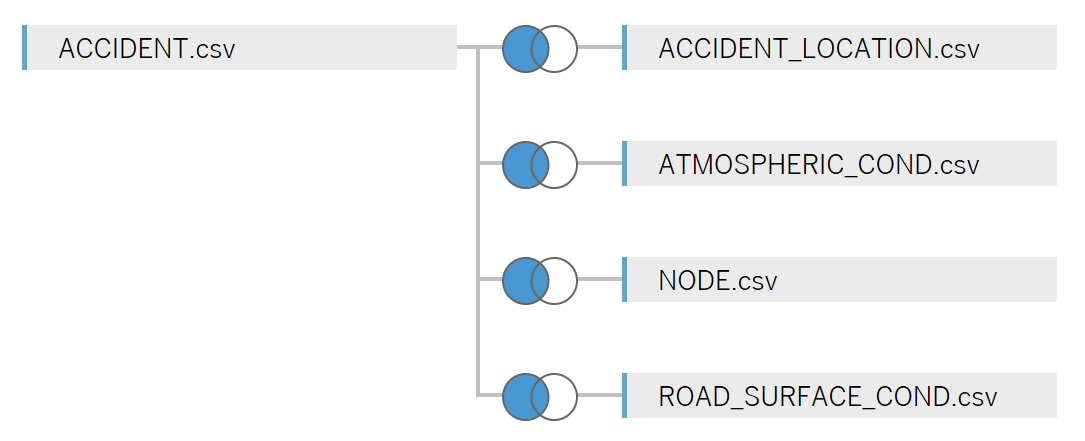
\includegraphics[scale=0.8]{leftouterjoin.png} 
	\end{center}
 	\label{fig:leftOuterJoin}
\caption{left outer joint structure}
\end{figure}


\section{Data Checking}
Tableau Public is a powerful tool for data wrangling, as well as data checking. In this section I will demonstrate the main step I performed for data checking. Because we will check the table which is generated in section \ref{JoinTable}. 
\label{dataChecking}
\subsection{Checking with Tableau Public}
After data wrangling, the data should be check to eliminate outlier. It is the process to detect and correct the inaccurate, incomplete, incorrect, or irrelevant part from the dataset. After 
The data exploration process can only be implemented after the data check, otherwise, the wrong data source will definitly lead the wrong results and conclusions. Data 

\section{Data Exploration}
\label{dataExploration}


\section{Conclusion}

\section{Reflection}




In this section, we define some important definitions and algorithms....
\begin{definition}
(Mixed Integer Programming)\\
In this report we consider a generic mixed-integer programming problem (MIP) in the following form
	\begin{align*}
	\text{(MIP)} \hspace{4mm} &\min \hspace{1.5mm}c^Tx \\
	s.t.\hspace{5mm} &Ax \geq b \\
	&x_j \in \mathbb{Z} \hspace{4mm} \forall j \in \mathcal{I}\\
	&x_j \in \mathbb{R} \hspace{4mm} \forall j \in \mathcal{N} \setminus \mathcal{I}\\
	\end{align*}
where the vector $b \in \mathbb{R}^m$ and the vector $c \in \mathbb{R}^n$ are input vectors.   $A$ is a input matrix of size $m \times n$, the variable input set $\mathcal{I} \subseteq \mathcal{N} = \lbrace 1,2,\dots,n\rbrace$. We denote $\mathcal{P}$ for this problem, which called a mixed-integer programming problem (MIP) with minimize objective function $c^Tx$ subject to the constraints $Ax \geq b$. Besides, some variables are restricted to integer values while the else of are restricted to real value. $S$ is a set of feasible solution if $S$ satisfy all the constraints in the problem. A vector $s^*$ with $s^* \in  S $ is called $optimal \, solution$ when $c^Tx_{s^*} \leq c^Tx_{s} \text{ for } \forall s \in S$.
When all of the variables are restricted to integer, the problem is called $pure integer linear program$(IP) for $\mathcal{I} = \mathcal{N}$. If there is no  integrality constraint, the program is called $linear program$
	\begin{align*}
	\text{(MIP)} \hspace{5mm} &\min \hspace{1.5mm}c^Tx \\
	s.t.\hspace{5mm} &Ax \geq b \\
	&x_j \in \mathbb{R} \hspace{4mm} \forall j \in \mathcal{N} \\
	\end{align*}
% ref: https://eprint.iacr.org/2012/676.pdf
% ref: Mixed-integer Linear Programming in the Analysis of Trivium and Ktantan
% ref: Reoptimization techniques in MIP Solvers

\citation{Mixed-Integer Programming}
\label{def_MIP}
\end{definition}

\begin{definition}
(LP-relaxation)\\
Lp $relaxation$ is obtained by removing all integrity constraints $ \mathcal{I} \leftarrow \emptyset$. LP-$relaxation$ is the foundation of LP-based branch-and-bound technology. As the searching space is increase by removing integrity restrictions, the optimal solution in MIP problem could not better than LP-$relaxation$, which is  $s_{MIP}^\ast \geq s_{LP}^\ast $. This means the optimal solution found in LP problem could provide a lower or prime bound for MIP problem.
\label{def_LP}
\end{definition}



\section{Input}
\begin{itemize}
    \item A MIP problem $\mathcal{P}^0$ with $n$ variables $x$,constraint set $C^0$ with an optimal solution $s^0$, where $s^0$ is a n-vector.
    \item A MIP problem $\mathcal{P}^1$ with $n$ variables $x$, constraint set $C^1$, such that $C^0 \subsetneq C^1$.
    
\end{itemize}							

\section{Output}
\begin{itemize}	
    \item An optimal solution $s^1$ to $\mathcal{P}^1$, where $s^1$ is a n-vector too.
\end{itemize}

\section{Pseudo Code}



\begin{algorithm}[H]
\SetAlgoLined
\DontPrintSemicolon
\KwIn{$ \mathcal{P}^1$ where $C^0 \subsetneq C^1$ and $\,  s^0$ , $k$}
\KwOut{ optimal solution $s^* \text{ to } \mathcal{P}^1 $}
\Begin{
	\eIf{$s^0\text{ is feasible to }\mathcal{P}^1$}{
			\textbf{return} $s^0$\;
 		} {
 			$\mathcal{I} \longleftarrow$ index set of integer or binary variables in $\mathcal{P}^1$\;
 			\For{$i$ in $\mathcal{I}$} {  
 				$\mathcal{P}^2 \longleftarrow$ create new variables $y_i$ and add it to $\mathcal{P}^1$: \tcp*[r]{add new variables} 
 				$\mathcal{P}^2 \longleftarrow $ add new constraints to $\mathcal{P}^2 \text{ : }y_i \geq x_i - s_i^0$ \tcp*[r]{add new constraints}
 				$\mathcal{P}^2 \longleftarrow $ add new constraints to $\mathcal{P}^2 \text{ : } y_i \geq s_i^0 - x_i$\;
 				%$\mathcal{P}^2 \longleftarrow $ add penalty function to $\mathcal{P}^2 \text{ : }\alpha \times y_j$\tcp*[r]{add penalty function} 
 			}
 			\If{the sense of $\mathcal{P}^2$ is not minimize }{
				change the sense of $\mathcal{P}^2$ to minimize\;	
 			}
 			stop gap $\longleftarrow 0.5$\;
 			\For{$l$ in $ \{k, k-1,\cdots, 0  \} $}{
 				$ \alpha \longleftarrow \alpha \times l $\;
				the coefficients of variables $y$ in $\mathcal{P}^2 \longleftarrow \alpha$\;			
 				\If{$l = 0$}{
 					stop gap $\longleftarrow 0.0$\;
 				}
 				$s^* \longleftarrow $ solving the sub-MIP problem to stop gap with reoptimization\;
 				}
 			\textbf{return} $s^*$\;
 			
	 	
 		}
}
 \caption{Solving Problem with Reoptimization}}{\label{alg_reop}
\end{algorithm}

\end{document}
